\documentclass[letter,onecolumn,12pt]{aiaa-tc}


\usepackage{color}
\usepackage[T1]{fontenc}
\usepackage[sc]{mathpazo}
\usepackage{caption}
\usepackage{subcaption}
\usepackage{blkarray}
\usepackage{paralist}
\usepackage{dsfont}
\usepackage{bm}
\usepackage{soul}
\usepackage{url}
\usepackage[cmex10]{amsmath}
%\usepackage[intlimits,cmex10]{amsmath}
\interdisplaylinepenalty=2500
\usepackage{amssymb}
\usepackage{floatflt}
\usepackage{epsfig,psfrag,graphicx,wrapfig}
%\usepackage[caption=false,font=footnotesize]{subfig}% subcaptions for subfigures
\usepackage[colorlinks]{hyperref}%  hyperlinks [must be loaded after dropping]
\usepackage{cite}
%\usepackage{refcheck}



% -----   NEW COMMANDS & ENVIRONMENTS   ----------------------------------------
%
\newcommand{\Lone}{\mathcal{L}_1}
\newcommand{\Linf}{\mathcal{L}_{\infty}}
\newcommand{\Lonenorm}[1]{\ensuremath{\left\Vert{#1}\right\Vert_{\mathcal{L}_1}}}
\newcommand{\Linfnorm}[1]{\ensuremath{\left\Vert{#1}\right\Vert_{\mathcal{L}_{\infty}}}}
\newcommand{\Linfnormt}[2]{\ensuremath{\left\Vert{#1}_{#2}\right\Vert_{\mathcal{L}_{\infty}}}}
\newcommand{\lonenorm}[1]{\ensuremath{\Vert{#1}\Vert_{\mathcal{L}_1}}}
\newcommand{\linfnorm}[1]{\ensuremath{\Vert{#1}\Vert_{\mathcal{L}_{\infty}}}}
\newcommand{\linfnormt}[2]{\ensuremath{\Vert{#1}_{#2}\Vert_{\mathcal{L}_{\infty}}}}
\newcommand{\Infnorm}[1]{\ensuremath{\left\Vert{#1}\right\Vert_{\infty}}}
%\newcommand{\Twonorm}[1]{\ensuremath{\left\Vert{#1}\right\Vert_{2}}}
\newcommand{\Twonorm}[1]{\ensuremath{\left\Vert{#1}\right\Vert}}
\newcommand{\Onenorm}[1]{\ensuremath{\left\Vert{#1}\right\Vert_{1}}}
\newcommand{\Abs}[1]{\ensuremath{\left|{#1}\right|}}
\newcommand{\infnorm}[1]{\ensuremath{\Vert{#1}\Vert_{\infty}}}
%\newcommand{\twonorm}[1]{\ensuremath{\Vert{#1}\Vert_{2}}}
\newcommand{\twonorm}[1]{\ensuremath{\Vert{#1}\Vert}}
\newcommand{\onenorm}[1]{\ensuremath{\Vert{#1}\Vert_{1}}}
\newcommand{\abs}[1]{\ensuremath{|{#1}|}}

\newcommand{\trace}[1]{\ensuremath{{\rm tr}\left[{#1}\right]}}
\newcommand{\Proj}[3]{\ensuremath{{\rm Proj}_{#1}({#2},{#3})}}
\newcommand{\Exp}[1]{\ensuremath{{\rm e}^{{#1}}}}
\newcommand{\Inv}[1]{\ensuremath{\left({#1}\right)^{-1}}}
\newcommand{\inv}[1]{\ensuremath{({#1})^{-1}}}

\newcommand{\drv}[2]{\frac{{\rm d}{#1}}{{\rm d}{#2}}}
\newcommand{\sat}[1]{\ensuremath{\operatorname{sat}\left({#1}\right)}}

\newcommand{\IR}{\mathds{R}}
\newcommand{\IZ}{\mathds{Z}}

\newcommand{\II}{\mathds{I}}
\newcommand{\IIn}[1]{\mathds{I}_{\bm{#1}}}

\newcommand{\matt}[1]{\begin{bmatrix}#1\end{bmatrix}}
\newcommand{\smatt}[1]{\left[\begin{smallmatrix}#1\end{smallmatrix}\right]}
\newcommand{\1}{1_n}
\newcommand{\col}{\operatorname{col}}
\newcommand{\card}{\operatorname{card}}

\newcommand{\Acal}{\mathcal{A}}
\newcommand{\Bcal}{\mathcal{B}}
\newcommand{\Ccal}{\mathcal{C}}
\newcommand{\Dcal}{\mathcal{D}}
\newcommand{\Ecal}{\mathcal{E}}
\newcommand{\Fcal}{\mathcal{F}}
\newcommand{\Gcal}{\mathcal{G}}
\newcommand{\Hcal}{\mathcal{H}}
\newcommand{\Ical}{\mathcal{I}}
\newcommand{\Jcal}{\mathcal{J}}
\newcommand{\Kcal}{\mathcal{K}}
\newcommand{\Lcal}{\mathcal{L}}
\newcommand{\Mcal}{\mathcal{M}}
\newcommand{\Ncal}{\mathcal{N}}
\newcommand{\Ocal}{\mathcal{O}}
\newcommand{\Pcal}{\mathcal{P}}
\newcommand{\Qcal}{\mathcal{Q}}
\newcommand{\Rcal}{\mathcal{R}}
\newcommand{\Scal}{\mathcal{S}}
\newcommand{\Tcal}{\mathcal{T}}
\newcommand{\Ucal}{\mathcal{U}}
\newcommand{\Vcal}{\mathcal{V}}
\newcommand{\Wcal}{\mathcal{W}}
\newcommand{\Xcal}{\mathcal{X}}
\newcommand{\Ycal}{\mathcal{Y}}
\newcommand{\Zcal}{\mathcal{Z}}
% ------------------------------------------------------------------------------


\graphicspath{{./figures/}}

\renewcommand{\baselinestretch}{1}



% ==============================================================================
% =====   PROPOSAL BEGINS HERE   ===============================================
% ==============================================================================
\begin{document}


\pagestyle{empty}
%==============================================================================
\section*{Executive Summary}  %<= 4,000 characters
%==============================================================================

%------------------------------------------------------------------------------
\textbf{\emph{Objective}:} The proposed research will develop an analytical framework for assessing the impact of miscommunication or low-connectivity conditions on the automated separation assurance of multiple cooperative airplanes sharing the same airspace. The Intergraded Separation Assurance In Low-Connectivity (iSEALC) framework is a solution of future high-density self-separating airflow concept envisioned by NextGen. iSEALC framework operates on the basis of cooperative multiple aircraft flying along their parameterized routes and sharing their state and intent information. The framework takes into account the switching topology and possibly degraded connectivity of the existing communication networks and performance characteristics of heterogeneous airplanes. The ultimate goal of the iSEALC framework is to provide a rapidly accessible and verifiable tool for assessing the separation guarantees of a given number of airplanes in a given ATC sector with degraded communication capabilities. The tool is  envisioned first to be integrated into existing mode of air traffic management as an advisory aid. At the second phase the fundamental coordination algorithms can be implemented onboard thus enabling automation of the route following and coordination. The technical challenges that will be addressed with iSEALC are the four subtopics of AFSC-1.5:
\vspace{-2mm}
\begin{itemize}
\setlength{\itemsep}{-4pt}
    \item formalize the failure space set of individual and integrated communication technologies,
    \item develop the separation violation metrics and a unified mitigation mechanism while operating under existing technological constraints,
    \item understand the impact of various types of communication constraints onto the separation assurance performance of the proposed unified strategy, and
    \item develop a mechanism by which communication disruptions and associated detection and mitigation strategies will guarantee separation assurance.
\end{itemize}
\vspace{-2mm}
%--------------------------  FIGURE  ------------------------------------------
\begin{wrapfigure}{r}{0.6\textwidth}
\centering
\vspace{-0mm}
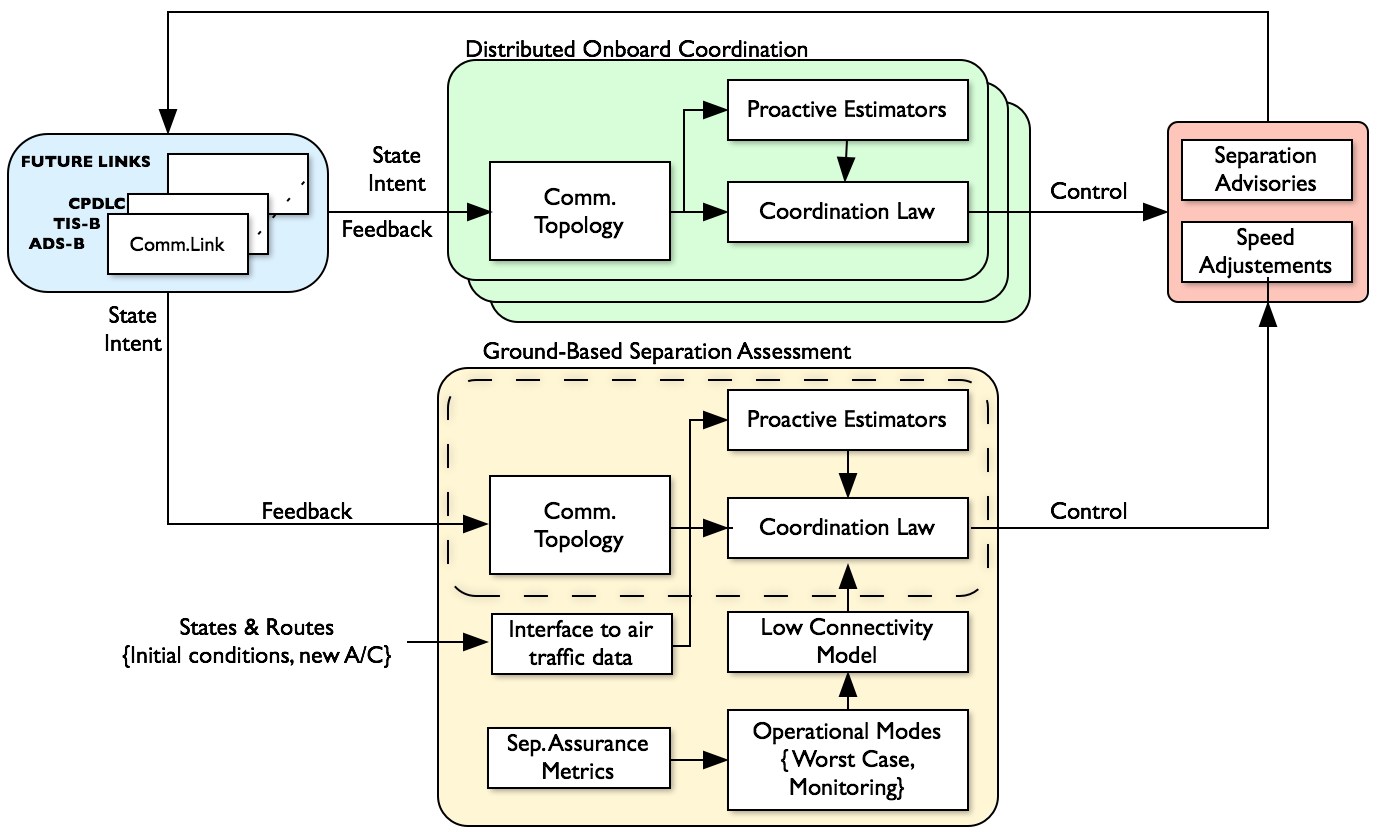
\includegraphics[angle=0,width=0.55\textwidth,]{iSEALC.png}
\caption*{\footnotesize iSEALC: \textbf{I}ntegrated \textbf{Se}paration \textbf{A}ssurance in \textbf{L}ow \textbf{C}onnectivity conditions.}
\label{fig:ISEALC}
\end{wrapfigure}
%------------------------------------------------------------------------------
\vspace{-1mm}

Research will build upon past expertise with the Coordinated Path Following (CPF) of Multiple UAVs project and the use of advanced adaptive control strategies to ensure a predictable response of a system of multiple heterogeneous airplanes sharing the same airspace in the presence of adverse communication conditions.The adverse communication conditions are defined by the degradation of the quality of communicated states which uniquely identify relative position and intent of the airplanes along their routes.

%This quality IS defined by the completeness of the state vector that specifies the state of the aircraft (position, speed course, trajectory angle, intent), the update rate of communicating the states across the network, and the network topology that might have disconnected segments. Special emphasis will be placed on the cumulative (over time) degradation of the communication topology and advanced algorithms of estimating of partially-communicated states across the time-varying network.

The proposed solution is based on transforming the key theoretical results of the CPF framework that is based on the 4D notion of trajectory representation that consists of the 3-dimensional analytical definition of path and the 1-dimensional velocity profile associated with the path. Multiple airplanes can be safely assigned to follow the same paths that intersect in space but are still separated in time.

%The CPF concept naturally fits the NextGen 4D notion of the airspace utilization; the CPF fundamental results are a perfect match for the key objectives of the nation-wide program.

\medskip

%------------------------------------------------------------------------------
\textbf{\emph{Expected Outcomes and Benefits}:} The expected outcome from this research effort is the iSEALC system (depicted in the figure). For a given ATC sector the system will ingest the current ATC status (class and geometry of the airspace segment, number and type of airplanes along with the assigned routes,  the communication capabilities of airborne assets and given ground support infrastructure) and produce a detailed report addressing possible separation assurance violations and remedies (controls).

%The report will address the following:
%\begin{itemize}
 %   \setlength{\itemsep}{-4pt}
%	\item possible violations of separation assurance with identification of specific routes and airplanes involved,
%   	\item proposed strategies to eliminate the separation faults expressed as adjustments of the speed control laws for each of the airplanes potentially involved in a collision,
%    	\item ability to submit this strategies onboard of airplanes for timely execution,
%    	\item ability to execute the iSEALC system algorithms either on the ground as an %assessment tool or to implement it onboard as a part of a pilot advisory system in a %distributed fashion to facilitate any desired level of automation.
%\end {itemize}

The following algorithms will be developed: $(i)$~the algorithms for detection of possible separation violations that identify the routes and the aircrafts involved; $(ii)$~the prioritization algorithms that produce a time-ordered sequence of possible violations; $(iii)$ - the recommended speed control laws capable to eliminate the violations; $(iv)$~the estimation algorithms that predict the position of neighboring airplanes which do not communicate their states. The main benefit will be a \emph{safer} automatic separation assurance system as envisioned under the NextGen concept in the 2025 time frame.

\medskip

%------------------------------------------------------------------------------
\textbf{\emph{Relevance to NASA Strategic Plan}:} The proposed research develops novel distributed control tools and methods that facilitate automation in airspace management while preserving robust separation assurance properties through scalability and cooperative computation. The proposed framework  assures safe operation under the communication technologies  and the air traffic mode of operation defined for NextGen. Besides compliance with current state of the art in NAS, the iSEALC framework perfectly matches the NextGen concept through applying its 4D-based trajectory representation, relying on distributed communication and computational capabilities that provide unprecedented scalable benefits and efficiency for the increased capacity of future NAS.
In particular, the proposed framework addresses the fundamental objectives of Subtopic~\mbox{AFCS-1.5} that is part of the System-Wide Safety Assurance Technologies Project (SSAT) and announced by the NASA Aeronautics Research Mission Directorate in support of NASA Strategic Goal~4 and Outcomes~4.1 and 4.2.

% ===== end Executive Summary   ===============================================



\clearpage
\thispagestyle{empty}
% =============================================================================
\tableofcontents
% =============================================================================



\clearpage
\pagestyle{plain}
\pagenumbering{arabic}
% =============================================================================
% === TECHNICAL SECTION (max 20 pages)   ======================================

% =============================================================================
\section{Objectives of the Proposed Research}
% =============================================================================

The main objective of this research is to develop assessment and mitigation tools and methods of automatic separation assurance which are capable to provide provable evidence of current level of safety of multiple cooperative airborne aircraft in the presence of degraded or intermittently lost communication. Degraded or even lost communication with air traffic controllers is one of the major reasons of fatal aircraft accidents\cite{Kochenderfer_2012}. The proposed  Intergraded Separation Assurance In Low-Connectivity (iSEALC) framework takes into account the switching topology and possibly degrading connectivity of the existing communication networks and performance characteristics of heterogeneous airplanes. The key enabling blocks of the iSEALC framework are the distributed coordination law and the set of proactive state estimators that enable self-separating cooperative flow of multiple aircraft in the presence of severely degraded communication.

The ultimate goal of the iSEALC framework is to provide a rapidly accessible and verifiable tool for assessing the separation guarantees of a given number of airplanes in a given ATC sector with degraded communication capabilities.  The tool is  envisioned first to be integrated into existing mode of airspace management as an advisory aid. At the second phase the fundamental coordination algorithms can be implemented onboard thus enabling automation of the route following and coordination. The technical challenges that will be addressed with iSEALC are the four subtopics of AFSC-1.5:
\vspace{-2mm}
\begin{itemize}
\setlength{\itemsep}{-4pt}
    \item formalize the failure space set of individual and integrated communication technologies,
    \item develop the separation violation metrics and a unified mitigation mechanism while operating under existing technological constraints,
    \item understand the impact of various types of communication constraints onto the separation assurance performance of the unified mitigation strategy, and
    \item develop a mechanism by which communication disruptions and associated detection and mitigation strategies will guarantee separation assurance.
\end{itemize}
\vspace{-2mm}

The adverse communication conditions are defined by the degradation of the quality of communicated states which uniquely identify relative position and intent of the airplanes along their routes. This quality is defined by the completeness of the delivered state vector that specifies the state of the aircraft (position, speed course, trajectory angle, intent), the update rate of communicating the states across the network, and the network topology that might have disconnected segments. Special emphasis will be placed on the cumulative (over time) loss of the communication and its impact on the degradation of separation assurance bounds. Addressing adverse effects of loss of communication, the research will also develop novel algorithms of estimating of partially-communicated states across the time-varying network.

We believe that integrating iSEALC architecture will be constructive in fundamentally improving situation awareness of all participants of the airflow process and improve overall safety of NAS operation.

% ===== end Objectives   ======================================================



% =============================================================================
\section{Technical Approach and Methodology}
% =============================================================================

% -----------------------------------------------------------------------------
\subsection{Background and Motivation }
% -----------------------------------------------------------------------------
It is estimated~\cite{FAA_ATO_2013} that there are about 7,000 aircraft occupying national airspace (NAS) at any given time. This number translates to almost 50,000 aircraft transiting the NAS everyday. The airspace is busy being constantly under stress and diverse set of adverse conditions coming from both the human and technological factors, as well as from the environment. Although the rate of air traffic control (ATC) errors of various categories remains low,  when taken cumulatively over a longer period of time, the dynamics of the ATC error rate in 2006 indicate a $68\%$  increase when compared to those reported in 1998~\cite{USAToday_2006}. According to FAA statistics, the number of reported operational errors increased by more than 50 percent between fiscal years 2009 and 2010. Thus, considering a constantly increasing air traffic density this positive trend in ATC and operational error rates might result in a serious increase in the number of accidents in near future. 

One of the parameters defining the safety of flight is the separation distance between aircraft. To help maintaining safe separation distances between aircraft, while under the control of ATC personnel, the Federal Aviation Administration (FAA) established minimum separation standards based on the aircraft's phase of flight and size. The ATC airspace surveillance infrastructure and controllers are responsible for providing instructions and advisories to pilots. 

Loss of standard separation (LOS) is an event when aircraft do not maintain the minimum distance apart. Despite significant efforts of a number of government authorities including the FAA and the National Transportation Safety Board (NTSB) the violation of LOS constraints still remains a significant safety concern~\cite{OIG_AR2013}. If unobserved or not timely and properly addressed the LOS encounter may result in near midair collisions and midair collisions (MAC) between aircraft in flight. Note, that most MAC incidents are direct results of LOS occurrence, while not every LOS event leads to a collision. On the same note, a MAC is an event observed and reported by a pilot that is based solely on a pilot's perspective, not on hard data. A loss of separation is based on hard data obtained by various instrumentation including radar data and their factual measurements that are thoroughly tracked.

First, it is worth illustrating the widespread of LOS events and the general nature of their causes. In January 2011, an operational error led to a LOS that resulted to a near mid-air collision  between a commercial airliner and two military aircraft near New York City. According to the NTSB\cite{OIG_AR2013}, who investigated the incident, at their closest proximity, the aircraft came within a mile of each other while 3 miles were required. There was no single point of failure identified as a result of the investigation but a sequence of steps that led to the LOS event. Since a number of instruments onboard and on the ground provided the telemetry of close proximity flight, the responsibility for the incident was assigned to the ATC personnel and crew.

On February 6, 2013  a number of  passenger planes were involved in a serious LOS incident in Finland~\cite{Vantaa_IR2013}.  Three civil aircraft were on approach to runway at Helsinki-Vantaa Airport; Norwegian Boeing-737, was on final approach, followed by a Flybe Nordic ATR, and a British Airways Airbus A320. A sequence of uncoordinated events between aircrafts and the ATC controller cased two sequential breaches of separation minima between each aircraft in pairs. Although there was no risk of collision according to the Safety Investigation Authority Finland~\cite{Vantaa_IR2013}, the LOS event was classified as a 'serious incident'.

On July 29th, 2011, a loss of separation occurred between two Boeing-737 aircrafts in the holding pattern at 93 miles south-west of Brisbane, Queensland\cite{Brisbane_ATSR2011}. The aircraft were inbound to Brisbane airport on the same air route, with a requirement to hold at BLAKA for sequencing. The air traffic controller did not identify that the sequence in which the two aircraft entered the holding pattern had changed, and twice assigned one of the aircraft descent through the flight level of another. The flight crew of lower flying aircraft identified the conflict and queried the controller, who then took action to recover the compromised separation situation. During the LOS event the separation reduced to 3.9 miles and 400 ft, while the required separation standard was 5 miles and 1000 ft. The Australian transport safety bureau identified that the controller was insufficiently trained, and had not consolidated effective control techniques for the sector, particularly for high-workload situations. 

The examples present very limited information taken primarily from the high-end instrumented aircraft and sufficient level of ATC support. However they do illustrate that the general practices and regulations tend to assign human error as the primary cause for the LOS incident. While the required human training and stuffing side is taken care by a number of FAA procedural changes and regulations\cite{OIG_AR2013} the lack of technology support is also evident. The number and variety of disparate sources of information characterizing excessively complex airspace require significant automation to be developed in support of airspace management. The algorithms of predicting potential LOS event for much longer time, possibly up to the entire flight duration, as a desired metric still need to be developed. Automatic assignment of en route and terminal approach sequencing of aircraft need to be automated and made dependent on the performance and equipage of the aircraft. The strategies accounting for the degraded communication among the ATC personnel on the ground and the airborne aircraft need to be developed.

At the same time, it also clear that there is no seldom single cause for an aircraft separation violation as it is usually a result of  a sequence of events triggered at a relatively late stage of close proximity encounter - last 3 to 10 minutes. This late stage of LOS detection is the result of lack of a unified system that would be able to ingest disparate data about all airborne vehicles and track the progression of all aircraft in the air while providing coordination command to the neighboring aircraft and shared access to this data to the entire fleet.

It is important to observe that although the current mode of airspace management assumes detailed knowledge of flight plan of every commercial aircraft that includes the detailed route and assigned speed profile, yet the LOS and MAC events happen. The probability of these events is unevenly shared between the en route and terminal airspace segments with the latter one contributing the vast majority of the occurrences; various sources including government authorities, industry and private sector provide inconsistent and therefore significantly ranging data, however the dominance of terminal airspace is obvious.

Furthermore, it is evident that ATC controllers have access to enormous amount of information obtained by disparate sources. Although supported by a number of technologies it is still their responsibility to fuse heterogeneous sources of information, interpret and keep updating the situational awareness so that their advisories to the crew are timely and unambiguous. On the other hand, the pilots have significant degree of freedom of interpretation of the advisories and the onboard instrumentation readings. Thus, being under stress of close proximity flight, they are often confused with frequent advisories~\cite{Kochenderfer_2012} given by the onboard systems (TACAS, ACAS, ACASx) on one hand and the instructions received from the ATC controllers on the other. When overloaded, the pilot is likely to make a mistake leading to fatal consequences. Therefore, although human errors are the biggest contributors to the LOS accidents, the current operational load of ATC controllers and pilots is approaching its limit. There is obvious need not only to automate the heterogeneous information fusion but also develop tools and methods that would detect the possibility of LOS way ahead of its occurrence. 

%As a result this separation of responsibilities, the most LOS events are classified as an  \emph{operational error} ,when the controller's actions caused the loss, while if the pilot's actions caused the LOS it is classified as a pilot \emph{deviation} and are not typically associated with errors caused by the situational awareness (instruments and algorithms) and data communication infrastructure.

Prevention of separation violation accidents becomes even more crucial in future airspace operations under the NextGen Air Transportation  System~\cite{NextGen_ConOps}. The NextGen concept envisions highly-integrated airspace operations in the 2025 time frame, necessary in order to cope with the rapid growth of air travel and operational diversity. The NextGen concept of operations includes high-density, all-weather, and self-separation operational concepts, and is also expected to allow mixed-capability aircraft to operate within the same airspace, including piloted aircraft and unmanned aircraft systems. Solution to this growing demand for high density self-separated airflow is in distributed automation that allows for desired scalability of algorithms and guarantees high robustness of the entire airspace management system to a failure of its single node.

%%Formulate the problem that was addressed by the old technologies. Highlight what is wrong with that setup. 

%ClosestProximity - The smallest distance ( point-to-point straight line in space) between two aircraft during an airborne loss of standard separation occurrence, regardless of geometry or percent of separation remaining.

%Measure of Compliance (MOC) - During a loss of standard separation occurrence involving radar separation minima for which recorded radar data is available, the greatest percentage of remaining separation (vertical or lateral) at the point of lowest separation conformance, as calculated by ATO Safety.

%Separation Conformance (SC) is based on the percentage of required separation that was maintained in both the vertical and horizontal dimensions. normalized euclidean distance. See FAATerminologyJO7210.633.pdf

%%Review existing approaches to the novel vision. Lincoln lab. the road from TCAS to ACAS and ACASx

%%Still what is the fundamental deficiency => Address separation asssurance only in the last minutes prioir to possible collision. Although very usefull it needs significant modification to enable analysisi of potential LOS accident from the beginning of the flight - injection point.

%%What we propose - deign nonintersecting in time trajectories, then DO precise automatic PF and coordinate with the rest over networks. 

%Before a solution can be formulated, it is necessary to obtain a quantitative definition of separation violation that is generally accepted among the investigators and researchers in this area.

%The authors of.....These generally accepted metrics will be used in the proposed research to quantify, identify, and predict separation violation events.

%An effective strategy is to monitor, identify and intervene at the different stages of a typical separation violation sequence by ... that collectively achieve separation assurance  guarantee.

In the context of automatic separation assurance as a part of the NextGen, the development of iSEALC framework will focus on ($i$) the analysis of  minimal necessary data to uniquely identify the state and intent of an aircraft in the air and the associated communication bandwidth, ($ii$) study nomenclature and limitations of current communication technologies from the perspective of their individual and cumulative contribution,($iii$) design novel algorithms to estimate the relative states of  neighboring aircraft in degraded communication conditions, and the contribution of these states into unified coordination control law, ($iv$) understand the limitations of separation performance of the designed cooperative control law as functions of the communication constraints and the aircraft performance limitations. Since the unified coordinated control law is constantly active throughout the entire flight, the iSEALC framework is persistently predicting the LOS event for each and all aircraft in the fleet. Hence, rather than intervening sequentially at the last moment and possibly leading to loss of separation and even mid air collision, the system will react as a normal feedback control law providing its desired performance and robust guarantees.

% -----------------------------------------------------------------------------
\subsection{Current Theoretical Developments and Results}
\label{subsec:current_develop}
% -----------------------------------------------------------------------------

The research team has successfully completed extensive research~\cite{xargay2012csm} in three key areas of this proposal: \emph{cooperative control of multiagent heterogeneous systems}, \emph{coordination performance degradation under adverse communication conditions}, and \emph{online estimation of partially known coordination states resulted from low-communication conditions}. Furthermore, the team made serious efforts to validate the key theoretical claims in a series of flight experiments involving multiple coordinated UAVs. The proposed research will build further upon these results. Therefore, an overview of the results is presented in this section.

\subsubsection{The Concept of Distributed Coordinaton }

...

\subsubsection{Coordination Performance Degradation Under Adverse Communication Conditions}

...

\subsubsection{Online estimation of partially known coordination states resulted from low-communication conditions}

% -----------------------------------------------------------------------------
\subsection{The Separation Assurance Framework}
\label{subsec:framework}
% -----------------------------------------------------------------------------

\subsubsection{Overview}
The architecture of iSEALC framework proposed in this research effort adopts the concept and methods of coordinated distributed path following that were introduced in the previous section. The iSEALC framework extends the developed  approach with algorithms and control schemes capable of rapidly identifying potential violations of separation assurance for a given set of heterogeneous aircrafts.

The framework can be initialized with a snapshot of current state of an airspace sector containing the number and type of aircrafts, their declared routes and nominal temporal assignments (speed profiles). As soon as the system is initialized the algorithms perform re-parameterization of the states, routes, and the speed control assignments in terms of primitives utilized by the CPF framework. Right at this stage the dimension of the separation assurance space significantly reduces thus making the solution of separation assurance task feasible to obtain in close to real-time pace.

Next, when utilized in ''the worst case scenario`` mode the system runs along the  parameterized paths with the predefined dynamics of aircrafts and evaluates the separation matrix (the matrix of separation distances for all pairs of aircrafts in the chosen airspace segment) in the presence of simulated adverse communication conditions caused by the capabilities of individual and integrated data broadcast systems. The best possible speed coordination law resulting from this worst case scenario implements the nominal PI-type control law developed in the CPF project; the interpretation of this result is analogous to the optimal control law in the task of robust control that maximizes the magnitude of disturbance caused by the low connectivity condition across all available communication channels.  The resulting separation matrix that represents the minimal separation distances between the $i$ and $j$ airplane pairs is naturally used as the metric for separation assurance. The minimum value of entries of this metric are the minimal distances nominally required by the FAA for each type of aircraft identified in possible violation of separation bounds. Thus when iSEALC is initialized or a new aircraft enters the considered segment the separation matrix is extended with the  bounding values assigned to corresponding pairs of aircrafts in the segment.

Obviously, that ``the worst case scenario'' would most likely result in significant number of panic pairs of the separation matrix. All of the panic pairs are the advisories for the ATC system and need to be monitored. To automate the monitoring process the same algorithms of iSEALC framework need to be utilized in ``monitoring`` mode when the system runs online and is fed by real data coming from all aircrafts in the considered segment. The varying communication conditions resulted from low connectivity or even loss of communication will necessarily result in adjusting the nominal speed control laws assigned to the aircrafts at the initialization stage. However, the PI architecture and the distributed nature of the speed coordination law will timely adjust the speed profiles of each aircraft in a potential separation violation condition. As long as the coordinated control law is not saturated (saturation bounds are different for each type of aircraft) the ''panicked`` mode will not be confirmed. In turn, if the control law of a specific aircraft is saturated then the panicked mode is confirmed and the corresponding advisory is given ahead of time to the ATC personnel with detailed specification of time to possible violation of separation bounds. This alarming condition still does not confirm the fact of collision as the onboard TACAS or ADS-B and other systems still provide pilots and onboard intelligence with sufficient information to avoid a collision.

To achieve the most effective mode of operation the iSEALC system can be integrated onboard of all aircrafts as an effective automated monitoring, advisory and control system. In this ''onboard`` mode the system relies on cooperative sharing of state and intent information across the entire fleet of aircrafts in a chosen airspace segment. When implemented onboard the system automatically adjusts the speed profiles of each and all aircrafts in the segment and guarantees that every vehicle follows its predefine path with the speed that guarantees the desired separation matrix. However the online mode becomes the most safety critical. To achieve significantly higher level of situational awareness we propose to develop and implement onboard an additional level of online estimators for all neighboring aircrafts states. This proactive estimators run in parallel with the coordination law, it estimates the states of the neighboring aircrafts while accounting for the degraded communication of states. The original coordination control law is thus extended with the estimated states of aircrafts nearby and thus provides higher robustness to low connectivity conditions.

In the following subsections we discuss some of the challenges and possible solutions for design and implementation of this technology.


\subsubsection{``Worst Case Scenario Architecture``}

...

\subsubsection{``Monitoring Mode Architecture''}

...

\subsubsection{``Onboard Architecture and Proactive Estimators''}

...
% -----------------------------------------------------------------------------
\subsection{Verification and Validation}
% -----------------------------------------------------------------------------

In order to validate the effectiveness and performance of the proposed research in preventing separation violation, the iSEALC system will be implemented in the Software-in-the-Loop~(SIL) and Hardware-In-The-Loop flight simulation. The team also proposes to transition the developed iSEALC framework to NASA LaRC or AMEs for implementation on the ATC simulators, which provides an actual airspace management environment to validate the developed technologies.


\subsubsection{Full-Scale Simulated Experiments}


\subsubsection{Technology Transition to NASA}

We propose to transition the developed framework to the facilities of

% ===== end Technical Approach and Methodology   ==============================



% =============================================================================
\section{Impact and Relevance of the Proposed Research}
% =============================================================================
A fundamental design requirement for the NextGen air traffic control system is a highly reliable and safe method for automating separation assurance. The iSEALC concept departs significantly from the current methods of separation assurance, which primarily focus on mid to short term identification and detection of loss of separation with simplistic mitigation strategies. In contrast the iSEALC architecture offers fundamentally new approach to separation assurance that is based on the 4D trajectory management, collaborative route planning, new separation modes that are based on distributed speed coordination, the system-wide network-based information management while preserving key safety requirements of the system in the degraded communication conditions. The objective of the proposed solution is to enable coordination of multiple aircraft through integration of a unified distributed coordinated control law that is constantly active throughout the entire flight. The iSEALC distributed framework of identical cooperative controllers is persistently predicting the LOS event for each and all aircraft in the fleet. Hence, rather than intervening sequentially at the last moment and possibly leading to the loss of separation and even mid air collision, the system reacts as a normal feedback control law providing its desired performance and robust guarantees. We hope that, given both the opportunity to contribute to the program and appropriate level of funding, the solutions proposed by us can be matured and transitioned from the flight of multiple R\&D UAVs to the real operational environment of NASA LaRC.

% ===== end Impact and Relevance   ============================================



% =============================================================================
\section{General Plan of Work}
% =============================================================================

% -----------------------------------------------------------------------------
\subsection{Key Milestones}
% -----------------------------------------------------------------------------

Within the next thirty-six months, if funded, the team of co-Is of this proposal will be working on ....

During the first year of research the analytical framework for the analysis of the individual and integrated failure space of communication technologies will be developed to facilitate a better understand-ing of the single fault (separation failure) detection and its probable spread across the network of air-planes.

During the second year of research an explicit set of communication failures will be formalized based on the performance characteristics of existing ground and airborne ATC solutions: ADS-B, GPS, TIS-B, and CPDLC. The realistic setups representing nominal and worst case communication scenarios will be built and assessed in software simulations, thus providing numerical illustrations of achievable separation assurance bounds.

During the last year of research a set of representative scenarios will be developed that can be tested using high fidelity hardware-in- the-loop simulations and flight tests utilizing advanced capabilities which are available at NPS and NASA facilities. The separation assurance bounds will be investigated during comprehensive flight-testing by using different autopilots and UAVs instrumented with advanced Real-Time (RT) control capability. To achieve verifiable flight test results we propose to utilize the capabilities of the Rapid Flight Control Prototyping System (RFCPS) that allows for onboard integration and RT execution of advanced algorithms.


% -----------------------------------------------------------------------------
\subsection{Management Structure}
% -----------------------------------------------------------------------------

Naira Hovakimyan will be the PI on this proposal. She will closely collaborate with


% -----------------------------------------------------------------------------
\subsection{Data-Sharing Plan}
% -----------------------------------------------------------------------------

All developed materials, including relevant literature reviews, algorithms, proofs, software, and design of specific experiments, will be shared with NASA by the co-Is of this proposal through regular bimonthly reports. All deliverables under the contract will be provided to NASA with unrestricted/unlimited rights. The co-Is will closely collaborate with NASA engineers, since the proposed work includes validation of the developed technologies on NASA research facilities. Therefore, the co-Is will ensure that all materials will be shared and adhere to NASA guidelines. Additionally, all computer code modules will be compatible with NASA software for further integration. In doing so, the co-Is strive to enhance the knowledge transfer and long-term value of the proposed work to NASA. Results will be submitted for publication to the AIAA~Guidance, Navigation, and Control Conference.

% ===== end General Plan of Work   ============================================


% ==============================================================================
% =====   PROPOSAL ENDS HERE   =================================================
% ==============================================================================



\clearpage
\pagenumbering{arabic}
% ==============================================================================
\bibliographystyle{ieeetran}
\bibliography{nasa_nra}
% ==============================================================================

\end{document} 